\documentclass[10pt]{beamer}
\usetheme{metropolis}
\usepackage{graphicx}
\usepackage{listings}
\usepackage{booktabs}
\usepackage{xcolor}
\usepackage{hyperref}
\usepackage{multicol}
\usepackage{tikz}

% ── Listing styles ──────────────────────────────────────────────
\definecolor{codebg}{HTML}{F5F5F5}
\definecolor{codegreen}{HTML}{2E7D32}
\definecolor{codegray}{HTML}{757575}
\definecolor{codepurple}{HTML}{7B1FA2}
\definecolor{codeblue}{HTML}{1565C0}

\lstdefinestyle{rstyle}{
  language=R,
  backgroundcolor=\color{codebg},
  basicstyle=\ttfamily\scriptsize,
  keywordstyle=\color{codeblue}\bfseries,
  stringstyle=\color{codegreen},
  commentstyle=\color{codegray}\itshape,
  numberstyle=\tiny\color{codegray},
  breaklines=true,
  frame=single,
  rulecolor=\color{codegray!30},
  showstringspaces=false,
  tabsize=2,
  morekeywords={library, ggplot, aes, geom_point, geom_line, theme_minimal,
                labs, tibble, mutate, filter, summarise, group_by, pipe}
}

\lstdefinestyle{pythonstyle}{
  language=Python,
  backgroundcolor=\color{codebg},
  basicstyle=\ttfamily\scriptsize,
  keywordstyle=\color{codeblue}\bfseries,
  stringstyle=\color{codegreen},
  commentstyle=\color{codegray}\itshape,
  numberstyle=\tiny\color{codegray},
  breaklines=true,
  frame=single,
  rulecolor=\color{codegray!30},
  showstringspaces=false,
  tabsize=4,
  morekeywords={import, from, as, pd, plt, sns, np}
}

% ── Metadata ────────────────────────────────────────────────────
\title{Why Visualize? The Case for Data Viz}
\subtitle{Workshop 1 --- Module 1}
\author{Prof.Asoc.\ Endri Raco}
\institute{Data Visualization for Data Scientists \\ UNYT Tirana}
\date{2025/26}

\begin{document}

% ================================================================
\begin{frame}
  \titlepage
\end{frame}

% ================================================================
\begin{frame}{Module Roadmap}
  \begin{enumerate}
    \item The information overload problem
    \item Historical masterpieces of data visualization
    \item Anscombe's quartet: why summary statistics lie
    \item The Datasaurus Dozen: a modern extension
    \item What makes visualization ``good''?
  \end{enumerate}

  \begin{exampleblock}{Learning Outcome}
    After this module you will be able to articulate \emph{why}
    visualization is an indispensable analytical tool, not merely
    a decorative afterthought.
  \end{exampleblock}
\end{frame}

% ================================================================
\section{The Information Overload Problem}
% ================================================================

\begin{frame}{We Are Drowning in Data}
  \begin{columns}[T]
    \begin{column}{0.55\textwidth}
      \begin{itemize}
        \item 2.5 quintillion bytes of data created \emph{daily}
        \item 90\% of the world's data generated in the last two years
        \item Corporate databases double every 12--18 months
        \item Human working memory: $7 \pm 2$ chunks
      \end{itemize}
    \end{column}
    \begin{column}{0.42\textwidth}
      \includegraphics[width=\textwidth]{figures/data_growth}
    \end{column}
  \end{columns}

  \begin{alertblock}{Pro-Tip}
    Raw tables with more than $\sim$20 rows are cognitively impenetrable.
    Visualization compresses dimensionality for the human visual cortex.
  \end{alertblock}
\end{frame}

% ================================================================
\begin{frame}{The Visual Bandwidth Advantage}
  \begin{columns}[T]
    \begin{column}{0.48\textwidth}
      \textbf{Table} (10 seconds to parse):\\[4pt]
      \begin{tabular}{lrr}
        \toprule
        Region & Q1 & Q2 \\
        \midrule
        North  & 142 & 189 \\
        South  & 98  & 115 \\
        East   & 205 & 178 \\
        West   & 167 & 201 \\
        \bottomrule
      \end{tabular}
    \end{column}
    \begin{column}{0.48\textwidth}
      \textbf{Chart} ($<$1 second to grasp):\\[4pt]
      \includegraphics[width=\textwidth]{figures/grouped_bar}
    \end{column}
  \end{columns}

  \vspace{6pt}
  \begin{exampleblock}{Data Insight}
    The visual cortex processes spatial patterns \textasciitilde60,000$\times$
    faster than sequential text. Charts exploit this parallel processing.
  \end{exampleblock}
\end{frame}

% ================================================================
\begin{frame}{Three Purposes of Visualization}
  \begin{enumerate}
    \item \textbf{Exploratory} --- discover patterns, generate hypotheses\\
          \emph{``What is going on in my data?''}
    \item \textbf{Explanatory} --- communicate known findings\\
          \emph{``Here is what I found and why it matters.''}
    \item \textbf{Confirmatory} --- validate or falsify expectations\\
          \emph{``Does the data support my model?''}
  \end{enumerate}

  \vspace{6pt}
  \begin{alertblock}{Pro-Tip}
    Most analysts jump straight to explanatory charts. Always begin with
    exploratory visualization --- you cannot explain what you have not
    first discovered.
  \end{alertblock}
\end{frame}

% ================================================================
\section{Historical Masterpieces}
% ================================================================

\begin{frame}{Charles Joseph Minard --- Napoleon's March (1869)}
  \begin{center}
    \includegraphics[width=0.92\textwidth]{figures/minard}
  \end{center}

  \begin{exampleblock}{Data Insight}
    Six variables on a single 2-D plane: army size, geographic position
    (lat/lon), direction of movement, temperature, and date. Tufte calls
    it ``the best statistical graphic ever drawn.''
  \end{exampleblock}
\end{frame}

% ================================================================
\begin{frame}{Florence Nightingale --- Coxcomb Diagram (1858)}
  \begin{columns}[T]
    \begin{column}{0.52\textwidth}
      \includegraphics[width=\textwidth]{figures/coxcomb}
    \end{column}
    \begin{column}{0.45\textwidth}
      \begin{itemize}
        \item Showed preventable deaths in the Crimean War
        \item Persuaded Parliament to fund sanitary reforms
        \item Area encoding for monthly mortality counts
        \item A pioneer of \emph{persuasive} data visualization
      \end{itemize}
    \end{column}
  \end{columns}
\end{frame}

% ================================================================
\begin{frame}{John Snow --- Cholera Map (1854)}
  \begin{columns}[T]
    \begin{column}{0.52\textwidth}
      \includegraphics[width=\textwidth]{figures/cholera_map}
    \end{column}
    \begin{column}{0.45\textwidth}
      \begin{itemize}
        \item Plotted cholera deaths as stacked bars on a street map
        \item Spatial clustering around the Broad Street pump
        \item Convinced authorities to remove the pump handle
        \item Foundational example of spatial epidemiology
      \end{itemize}
    \end{column}
  \end{columns}

  \begin{exampleblock}{Data Insight}
    Snow's map is arguably the first GIS analysis---a point pattern
    overlaid on a geographic reference layer, centuries before ArcGIS.
  \end{exampleblock}
\end{frame}

% ================================================================
\begin{frame}{W.E.B.\ Du Bois --- Data Portraits (1900)}
  \begin{columns}[T]
    \begin{column}{0.48\textwidth}
      \includegraphics[width=\textwidth]{figures/dubois}
    \end{column}
    \begin{column}{0.48\textwidth}
      \begin{itemize}
        \item Presented at the Paris Exposition, 1900
        \item Visualized African-American economic progress
        \item Strikingly modern design: spiral charts, proportional areas
        \item Data as a tool of social justice and advocacy
      \end{itemize}
    \end{column}
  \end{columns}
\end{frame}

% ================================================================
\begin{frame}{Lessons from the Masters}
  \centering
  \begin{tabular}{llp{4.5cm}}
    \toprule
    \textbf{Practitioner} & \textbf{Year} & \textbf{Key Innovation} \\
    \midrule
    Minard       & 1869 & Multivariate narrative on a single plane \\
    Nightingale  & 1858 & Persuasive polar-area chart \\
    Snow         & 1854 & Spatial point-pattern overlay \\
    Du Bois      & 1900 & Design as social advocacy \\
    \bottomrule
  \end{tabular}

  \vspace{8pt}
  Every masterpiece combined \textbf{data integrity} with
  \textbf{design clarity} and a \textbf{compelling narrative}.
\end{frame}

% ================================================================
\section{Anscombe's Quartet}
% ================================================================

\begin{frame}{The Trap of Summary Statistics}
  \begin{columns}[T]
    \begin{column}{0.48\textwidth}
      Four datasets, \emph{identical} descriptive statistics:
      \begin{itemize}
        \item $\bar{x} = 9.0$, \; $\bar{y} = 7.50$
        \item $\sigma_x = 3.32$, \; $\sigma_y = 2.03$
        \item $r = 0.816$
        \item Regression: $y = 3.0 + 0.5x$
      \end{itemize}
    \end{column}
    \begin{column}{0.48\textwidth}
      \includegraphics[width=\textwidth]{figures/anscombe_table}
    \end{column}
  \end{columns}

  \vspace{6pt}
  \textbf{Question}: If every statistical summary is identical,
  are the datasets interchangeable?
\end{frame}

% ================================================================
\begin{frame}{Anscombe's Quartet --- Visualized}
  \begin{center}
    \includegraphics[width=0.82\textwidth]{figures/anscombe_scatter}
  \end{center}

  \begin{exampleblock}{Data Insight}
    Dataset I is linear; II is curvilinear; III has a single outlier
    pulling the regression; IV has a single influential point.
    \textbf{Always plot your data.}
  \end{exampleblock}
\end{frame}

% ================================================================
\begin{frame}[fragile]{Anscombe's Quartet in R}
  \begin{columns}[T]
    \begin{column}{0.52\textwidth}
\begin{lstlisting}[style=rstyle]
# Anscombe's quartet is built into R
data(anscombe)

# Reshape to long format
library(tidyverse)
anscombe_long <- anscombe |>
  pivot_longer(
    everything(),
    names_to = c(".value", "set"),
    names_pattern = "(.)(.)"
  )

# Plot all four datasets
ggplot(anscombe_long,
       aes(x = x, y = y)) +
  geom_point(size = 2) +
  geom_smooth(method = "lm",
              se = FALSE,
              color = "steelblue") +
  facet_wrap(~set, ncol = 2) +
  theme_minimal()
\end{lstlisting}
    \end{column}
    \begin{column}{0.45\textwidth}
      \includegraphics[width=\textwidth]{figures/anscombe_r_output}
    \end{column}
  \end{columns}
\end{frame}

% ================================================================
\begin{frame}[fragile]{Anscombe's Quartet in Python}
  \begin{columns}[T]
    \begin{column}{0.52\textwidth}
\begin{lstlisting}[style=pythonstyle]
import seaborn as sns
import matplotlib.pyplot as plt

# Load built-in Anscombe data
df = sns.load_dataset("anscombe")

# FacetGrid with regression
g = sns.lmplot(
    data=df,
    x="x", y="y",
    col="dataset",
    col_wrap=2,
    ci=None,
    height=3,
    scatter_kws={"s": 40}
)
g.set_titles("Dataset {col_name}")
plt.tight_layout()
plt.savefig("anscombe.png", dpi=150)
\end{lstlisting}
    \end{column}
    \begin{column}{0.45\textwidth}
      \includegraphics[width=\textwidth]{figures/anscombe_py_output}
    \end{column}
  \end{columns}
\end{frame}

% ================================================================
\section{The Datasaurus Dozen}
% ================================================================

\begin{frame}{Beyond Anscombe: The Datasaurus Dozen (2017)}
  \begin{center}
    \includegraphics[width=0.85\textwidth]{figures/datasaurus}
  \end{center}

  \begin{exampleblock}{Data Insight}
    Matejka \& Fitzmaurice (2017) generated 13 datasets with
    \emph{identical} means, standard deviations, and correlations
    --- yet wildly different shapes, including a dinosaur.
    Reference: \emph{CHI 2017 Proceedings}.
  \end{exampleblock}
\end{frame}

% ================================================================
\begin{frame}[fragile]{Datasaurus in R}
  \begin{columns}[T]
    \begin{column}{0.52\textwidth}
\begin{lstlisting}[style=rstyle]
# Install datasauRus package
# install.packages("datasauRus")
library(datasauRus)
library(ggplot2)

# All 13 datasets share the
# same summary statistics
ggplot(datasaurus_dozen,
       aes(x = x, y = y)) +
  geom_point(alpha = 0.6,
             size = 0.8) +
  facet_wrap(~dataset,
             ncol = 5) +
  theme_minimal(base_size = 8) +
  labs(
    title = "Same Stats,
             Different Graphs",
    caption = "datasauRus package"
  )
\end{lstlisting}
    \end{column}
    \begin{column}{0.45\textwidth}
      \includegraphics[width=\textwidth]{figures/datasaurus}
    \end{column}
  \end{columns}
\end{frame}

% ================================================================
\begin{frame}[fragile]{Datasaurus in Python}
  \begin{columns}[T]
    \begin{column}{0.52\textwidth}
\begin{lstlisting}[style=pythonstyle]
# pip install datasaurus
# or use the CSV directly
import pandas as pd
import seaborn as sns
import matplotlib.pyplot as plt

url = ("https://raw.githubusercontent"
       ".com/jumpingrivers/"
       "datasauRus/main/inst/"
       "extdata/DatasaurusDozen"
       "-long.tsv")
df = pd.read_csv(url, sep="\t")

g = sns.FacetGrid(
    df, col="dataset",
    col_wrap=5, height=2
)
g.map(plt.scatter, "x", "y",
      s=5, alpha=0.6)
g.set_titles("{col_name}")
plt.tight_layout()
plt.savefig("datasaurus.png",
            dpi=150)
\end{lstlisting}
    \end{column}
    \begin{column}{0.45\textwidth}
      \includegraphics[width=\textwidth]{figures/datasaurus}
    \end{column}
  \end{columns}
\end{frame}

% ================================================================
\begin{frame}[fragile]{Verify: Same Statistics, Different Pictures}
  \begin{columns}[T]
    \begin{column}{0.48\textwidth}
      \textbf{R verification:}
\begin{lstlisting}[style=rstyle]
library(dplyr)
datasaurus_dozen |>
  group_by(dataset) |>
  summarise(
    mean_x = mean(x),
    mean_y = mean(y),
    sd_x   = sd(x),
    sd_y   = sd(y),
    cor_xy = cor(x, y)
  )
\end{lstlisting}
    \end{column}
    \begin{column}{0.48\textwidth}
      \textbf{Python verification:}
\begin{lstlisting}[style=pythonstyle]
summary = df.groupby(
    "dataset"
).agg(
    mean_x=("x", "mean"),
    mean_y=("y", "mean"),
    sd_x=("x", "std"),
    sd_y=("y", "std"),
    cor_xy=("x", lambda s:
      s.corr(
        df.loc[s.index, "y"]
      ))
)
print(summary.round(2))
\end{lstlisting}
    \end{column}
  \end{columns}

  \vspace{4pt}
  \begin{alertblock}{Pro-Tip}
    Every dataset returns $\bar{x} \approx 54.3$, $\bar{y} \approx 47.8$,
    $\sigma_x \approx 16.8$, $\sigma_y \approx 26.9$, $r \approx -0.06$.
    \textbf{Never trust statistics without visualization.}
  \end{alertblock}
\end{frame}

% ================================================================
\section{What Makes Visualization ``Good''?}
% ================================================================

\begin{frame}{Edward Tufte's Principles of Graphical Excellence}
  \begin{columns}[T]
    \begin{column}{0.65\textwidth}
      A visualization achieves \textbf{graphical excellence} when it:
      \begin{enumerate}
        \item Shows the data clearly and accurately
        \item Induces thinking about \emph{substance}, not method
        \item Avoids distortion of what the data reveal
        \item Presents many numbers in a small space
      \end{enumerate}
    \end{column}
    \begin{column}{0.32\textwidth}
      \includegraphics[width=\textwidth]{figures/tufte_book}
    \end{column}
  \end{columns}

  \vspace{6pt}
  \emph{``Excellence in statistical graphics consists of complex ideas
  communicated with clarity, precision, and efficiency.''}\\
  \hfill--- Tufte (1983), p.~51
\end{frame}

% ================================================================
\begin{frame}{Alberto Cairo's Truthful Art Framework}
  A visualization should be:
  \begin{enumerate}
    \item \textbf{Truthful} --- based on thorough, honest research
    \item \textbf{Functional} --- constitutes an accurate depiction
    \item \textbf{Beautiful} --- attractive and intriguing
    \item \textbf{Insightful} --- reveals evidence not detectable otherwise
    \item \textbf{Enlightening} --- changes minds if warranted by evidence
  \end{enumerate}

  \vspace{6pt}
  \begin{exampleblock}{Data Insight}
    Cairo's framework resolves the false dichotomy between ``pretty'' and
    ``accurate.'' Effective visualization is \emph{simultaneously} both.
  \end{exampleblock}
\end{frame}

% ================================================================
\begin{frame}{The Data-Ink Ratio}
  \begin{center}
    \Large
    $\displaystyle \text{Data-Ink Ratio} = \frac{\text{Ink used to represent data}}{\text{Total ink on the graphic}}$
  \end{center}

  \vspace{6pt}
  \begin{columns}[T]
    \begin{column}{0.48\textwidth}
      \textbf{Low ratio (bad):}
      \begin{itemize}
        \item Heavy gridlines
        \item 3-D effects, drop shadows
        \item Decorative images
        \item Redundant legends
      \end{itemize}
    \end{column}
    \begin{column}{0.48\textwidth}
      \textbf{High ratio (good):}
      \begin{itemize}
        \item Minimal non-data ink
        \item Direct labels
        \item Whitespace as structure
        \item Every mark = a data point
      \end{itemize}
    \end{column}
  \end{columns}
\end{frame}

% ================================================================
\begin{frame}{Chart Junk: What to Avoid}
  \begin{center}
    \includegraphics[width=0.8\textwidth]{figures/chartjunk}
  \end{center}

  Tufte's catalogue of chart junk:
  \begin{itemize}
    \item Unnecessary 3-D effects and perspective distortion
    \item Moir\'{e} vibration patterns and heavy crosshatching
    \item Decorative ``ducks'' that distract from data
    \item Over-designed grids that compete with data points
  \end{itemize}
\end{frame}

% ================================================================
\begin{frame}{Good vs.\ Bad: A Before/After}
  \begin{columns}[T]
    \begin{column}{0.48\textwidth}
      \textbf{Before (Cluttered)}
      \includegraphics[width=\textwidth]{figures/before_cluttered}

      Issues: 3-D bars, gradient fills, rotated axis labels,
      unnecessary legend box.
    \end{column}
    \begin{column}{0.48\textwidth}
      \textbf{After (Clean)}
      \includegraphics[width=\textwidth]{figures/after_clean}

      Fixes: 2-D horizontal bars, direct labels,
      sorted by value, minimal grid.
    \end{column}
  \end{columns}
\end{frame}

% ================================================================
\begin{frame}{The Lie Factor}
  \begin{center}
    \Large
    $\displaystyle \text{Lie Factor} = \frac{\text{Effect shown in graphic}}{\text{Effect in data}}$
  \end{center}

  \vspace{6pt}
  \begin{itemize}
    \item A lie factor of 1.0 = perfect honesty
    \item Lie factor $>$ 1.05 or $<$ 0.95 = visual deception
    \item Common sources: truncated axes, area-encoded bars, perspective
  \end{itemize}

  \begin{alertblock}{Pro-Tip}
    Always check: if the data increased by 50\%, does the visual
    encoding (height, area, volume) also increase by exactly 50\%?
  \end{alertblock}
\end{frame}

% ================================================================
\begin{frame}{Munzner's Nested Model for Visualization Design}
  \begin{center}
    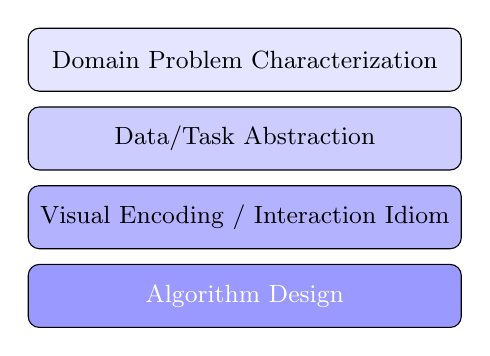
\begin{tikzpicture}[
      box/.style={draw, rounded corners, minimum width=5.5cm,
                  minimum height=0.8cm, align=center, font=\small}
    ]
      \node[box, fill=blue!10]  at (0, 3.0) {Domain Problem Characterization};
      \node[box, fill=blue!20]  at (0, 2.0) {Data/Task Abstraction};
      \node[box, fill=blue!30]  at (0, 1.0) {Visual Encoding / Interaction Idiom};
      \node[box, fill=blue!40, text=white] at (0, 0.0) {Algorithm Design};
    \end{tikzpicture}
  \end{center}

  \vspace{4pt}
  Each layer validates the layer above it. Errors at outer layers
  propagate inward and cannot be fixed by inner-layer improvements.
\end{frame}

% ================================================================
\section{Putting It Together}
% ================================================================

\begin{frame}{The Visualization Design Checklist}
  Before publishing any chart, verify:
  \begin{enumerate}
    \item \textbf{Purpose}: What question does this answer?
    \item \textbf{Data integrity}: Does it accurately represent the data?
    \item \textbf{Audience}: Who will read this and what do they need?
    \item \textbf{Clarity}: Can the message be grasped in $<$ 5 seconds?
  \end{enumerate}

  \vspace{6pt}
  \begin{exampleblock}{Data Insight}
    Effective visualization sits at the intersection of
    \textbf{data science} (what is true),
    \textbf{design} (what is clear), and
    \textbf{storytelling} (what is compelling).
  \end{exampleblock}
\end{frame}

% ================================================================
\begin{frame}[fragile]{Your First Plot in R (Preview)}
  \begin{columns}[T]
    \begin{column}{0.52\textwidth}
\begin{lstlisting}[style=rstyle]
library(ggplot2)

# Built-in mpg dataset
ggplot(mpg,
       aes(x = displ,
           y = hwy,
           color = class)) +
  geom_point(size = 2,
             alpha = 0.7) +
  labs(
    title = "Engine Size vs
             Highway MPG",
    x = "Displacement (L)",
    y = "Highway MPG"
  ) +
  theme_minimal()
\end{lstlisting}
    \end{column}
    \begin{column}{0.45\textwidth}
      \includegraphics[width=\textwidth]{figures/mpg_r_output}
    \end{column}
  \end{columns}
\end{frame}

% ================================================================
\begin{frame}[fragile]{Your First Plot in Python (Preview)}
  \begin{columns}[T]
    \begin{column}{0.52\textwidth}
\begin{lstlisting}[style=pythonstyle]
import seaborn as sns
import matplotlib.pyplot as plt

# Built-in mpg dataset
mpg = sns.load_dataset("mpg")

sns.scatterplot(
    data=mpg,
    x="displacement",
    y="mpg",
    hue="origin",
    alpha=0.7,
    s=50
)
plt.title("Displacement vs MPG")
plt.xlabel("Displacement (cu in)")
plt.ylabel("Miles per Gallon")
plt.tight_layout()
plt.savefig("first_plot.png",
            dpi=150)
\end{lstlisting}
    \end{column}
    \begin{column}{0.45\textwidth}
      \includegraphics[width=\textwidth]{figures/mpg_py_output}
    \end{column}
  \end{columns}
\end{frame}

% ================================================================
\begin{frame}{Key Takeaways}
  \begin{enumerate}
    \item \textbf{Visualization is analysis}, not decoration --- it reveals
          structure that summary statistics hide (Anscombe, Datasaurus).
    \item \textbf{Historical precedent}: Minard, Nightingale, Snow, Du Bois
          used visualization to change policy and save lives.
    \item \textbf{Principled design} matters: data-ink ratio, lie factor,
          and the nested model provide rigorous evaluation criteria.
    \item \textbf{R and Python} are equally capable --- this course teaches
          both in parallel so you choose the right tool for the context.
  \end{enumerate}
\end{frame}

% ================================================================
\begin{frame}{Essential Readings for This Module}
  \begin{itemize}
    \item Tufte, E.~R. (1983). \emph{The Visual Display of Quantitative
          Information}, Chapter~1.
    \item Cairo, A. (2012). \emph{The Functional Art}, Introduction \&
          Chapter~1.
    \item Anscombe, F.~J. (1973). ``Graphs in Statistical Analysis,''
          \emph{The American Statistician}, 27(1), 17--21.
    \item Matejka, J. \& Fitzmaurice, G. (2017). ``Same Stats, Different
          Graphs,'' \emph{CHI 2017}.
  \end{itemize}

  \vspace{6pt}
  \textbf{Next Module}: Tufte's Principles of Graphical Excellence (W01-M02)
\end{frame}

\end{document}
